Sei $F$ die Antriebskraft, $m_\mathrm{L}$ die Masse der Lokomotive, $n$ die Anzahl Wagen und $m_\mathrm{W}$ die Masse eines Wagens.

\begin{center}
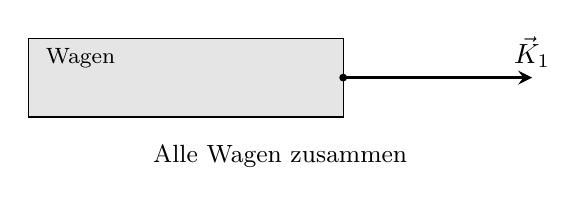
\begin{tikzpicture}[>=stealth]
 \draw[fill=gray!20] (-2,-0.5) rectangle (2,0.5);
 \node[anchor=north west, font=\footnotesize] at (-2,0.5) {\nWO\ Wagen};
 \draw[->, very thick] (2,0) -- (4.4,0);
 \fill (2,0) circle (0.05);
 \node[above] at (4.4,0) {$\vec K_1$};
 \node[font=\small] at (1.2,-1) {Alle Wagen zusammen};
\end{tikzpicture}
\hspace{1cm}
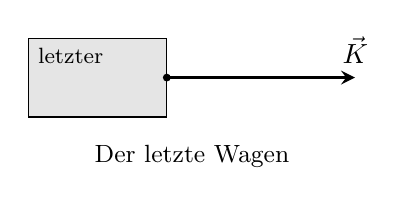
\begin{tikzpicture}[>=stealth]
 \draw[fill=gray!20] (-0.88,-0.5) rectangle (0.88,0.5);
 \node[anchor=north west, font=\footnotesize] at (-0.88,0.5) {letzter};
 \draw[->, very thick] (0.88,0) -- (3.27,0);
 \fill (0.88,0) circle (0.05);
 \node[above] at (3.27,0) {$\vec K_{\nWO}$};
 \node[font=\small] at (1.2,-1) {Der letzte Wagen};
\end{tikzpicture}
\end{center}
Gewichtskraft und Normalkraft heben sich auf; sie sind weggelassen. Die beiden Bilder haben verschiedene Massstäbe.

\begin{abcliste}
\abc
Der ganze Zug als ein System: Die Antriebskraft beschleunigt die gesamte Masse.
\begin{align}
 a &= \aF \\
   &= \frac{\FA}{\mLo+\nWO\cdot\mWg} \\
   &= \a \approx \result{\aP{0}{2}}
\end{align}

\abc
Eine Kupplung zieht alle Wagen hinter ihr, und nur diese: deren Masse mal die Beschleunigung. Die erste Kupplung zieht alle \nWO\ Wagen:
\begin{align}
 K_1 &= \KaF \\
   &= \nWO\cdot\mWg\cdot\a \\
   &= \Ka \approx \result{\KaP{3}{2}}
\end{align}

\abc
Die letzte Kupplung zieht nur den letzten Wagen:
\begin{align}
 K_{\nWO} &= \KbF \\
   &= \mWg\cdot\a \\
   &= \Kb \approx \result{\KbP{3}{2}}
\end{align}
Die vorderen Kupplungen tragen am meisten: Dort reissen Züge auseinander.
\end{abcliste}
